\documentclass[12pt]{article}
\usepackage[margin=1in]{geometry}
\usepackage{listings}
\usepackage{graphicx}
\usepackage{float}
\usepackage{color} %red, green, blue, yellow, cyan, magenta, black, white
\definecolor{mygreen}{RGB}{28,172,0} % color values Red, Green, Blue
\definecolor{mylilas}{RGB}{170,55,241}

\setlength{\parskip}{1em}

\lstset{language=Matlab,%
    %basicstyle=\color{red},
    breaklines=true,%
    morekeywords={matlab2tikz},
    keywordstyle=\color{blue},%
    morekeywords=[2]{1}, keywordstyle=[2]{\color{black}},
    identifierstyle=\color{black},%
    stringstyle=\color{mylilas},
    commentstyle=\color{mygreen},%
    showstringspaces=false,%without this there will be a symbol in the places where there is a space
    numbers=left,%
    numberstyle={\tiny \color{black}},% size of the numbers
    numbersep=9pt, % this defines how far the numbers are from the text
    emph=[1]{for,end,break},emphstyle=[1]\color{red}, %some words to emphasise
    %emph=[2]{word1,word2}, emphstyle=[2]{style},    
}


\title{Assignment 1, COMP4702}
\author{Roy Portas}
\date{\today}

\begin{document}

\begin{titlepage}
    \maketitle
\end{titlepage}

\section*{Question 1.2}

The first column of the data is the date, the second column appears to be a
unique ID for each entry.

The third column contains numbers between 25 and 30, this is possibly a
temperature in degrees. The values also change gradually which seems correct
for the given time intervals

The fourth column contains numbers between 26 and around 50000. If this is
plotted against the ID field, it produces a line.

The fifth column contains numbers between 7.3 and 8.3, with a mean of 7.846 and
a standard StdDev of 0.142. This suggests that the value doesn't change much.

It could possibly be weather data, containing temperature, humidity, etc.

\section*{Question 1.6}

\lstinputlisting[language=Matlab]{../../pracs/week2/q6.m}

\section*{Question 2.1}

\begin{figure}[H]
    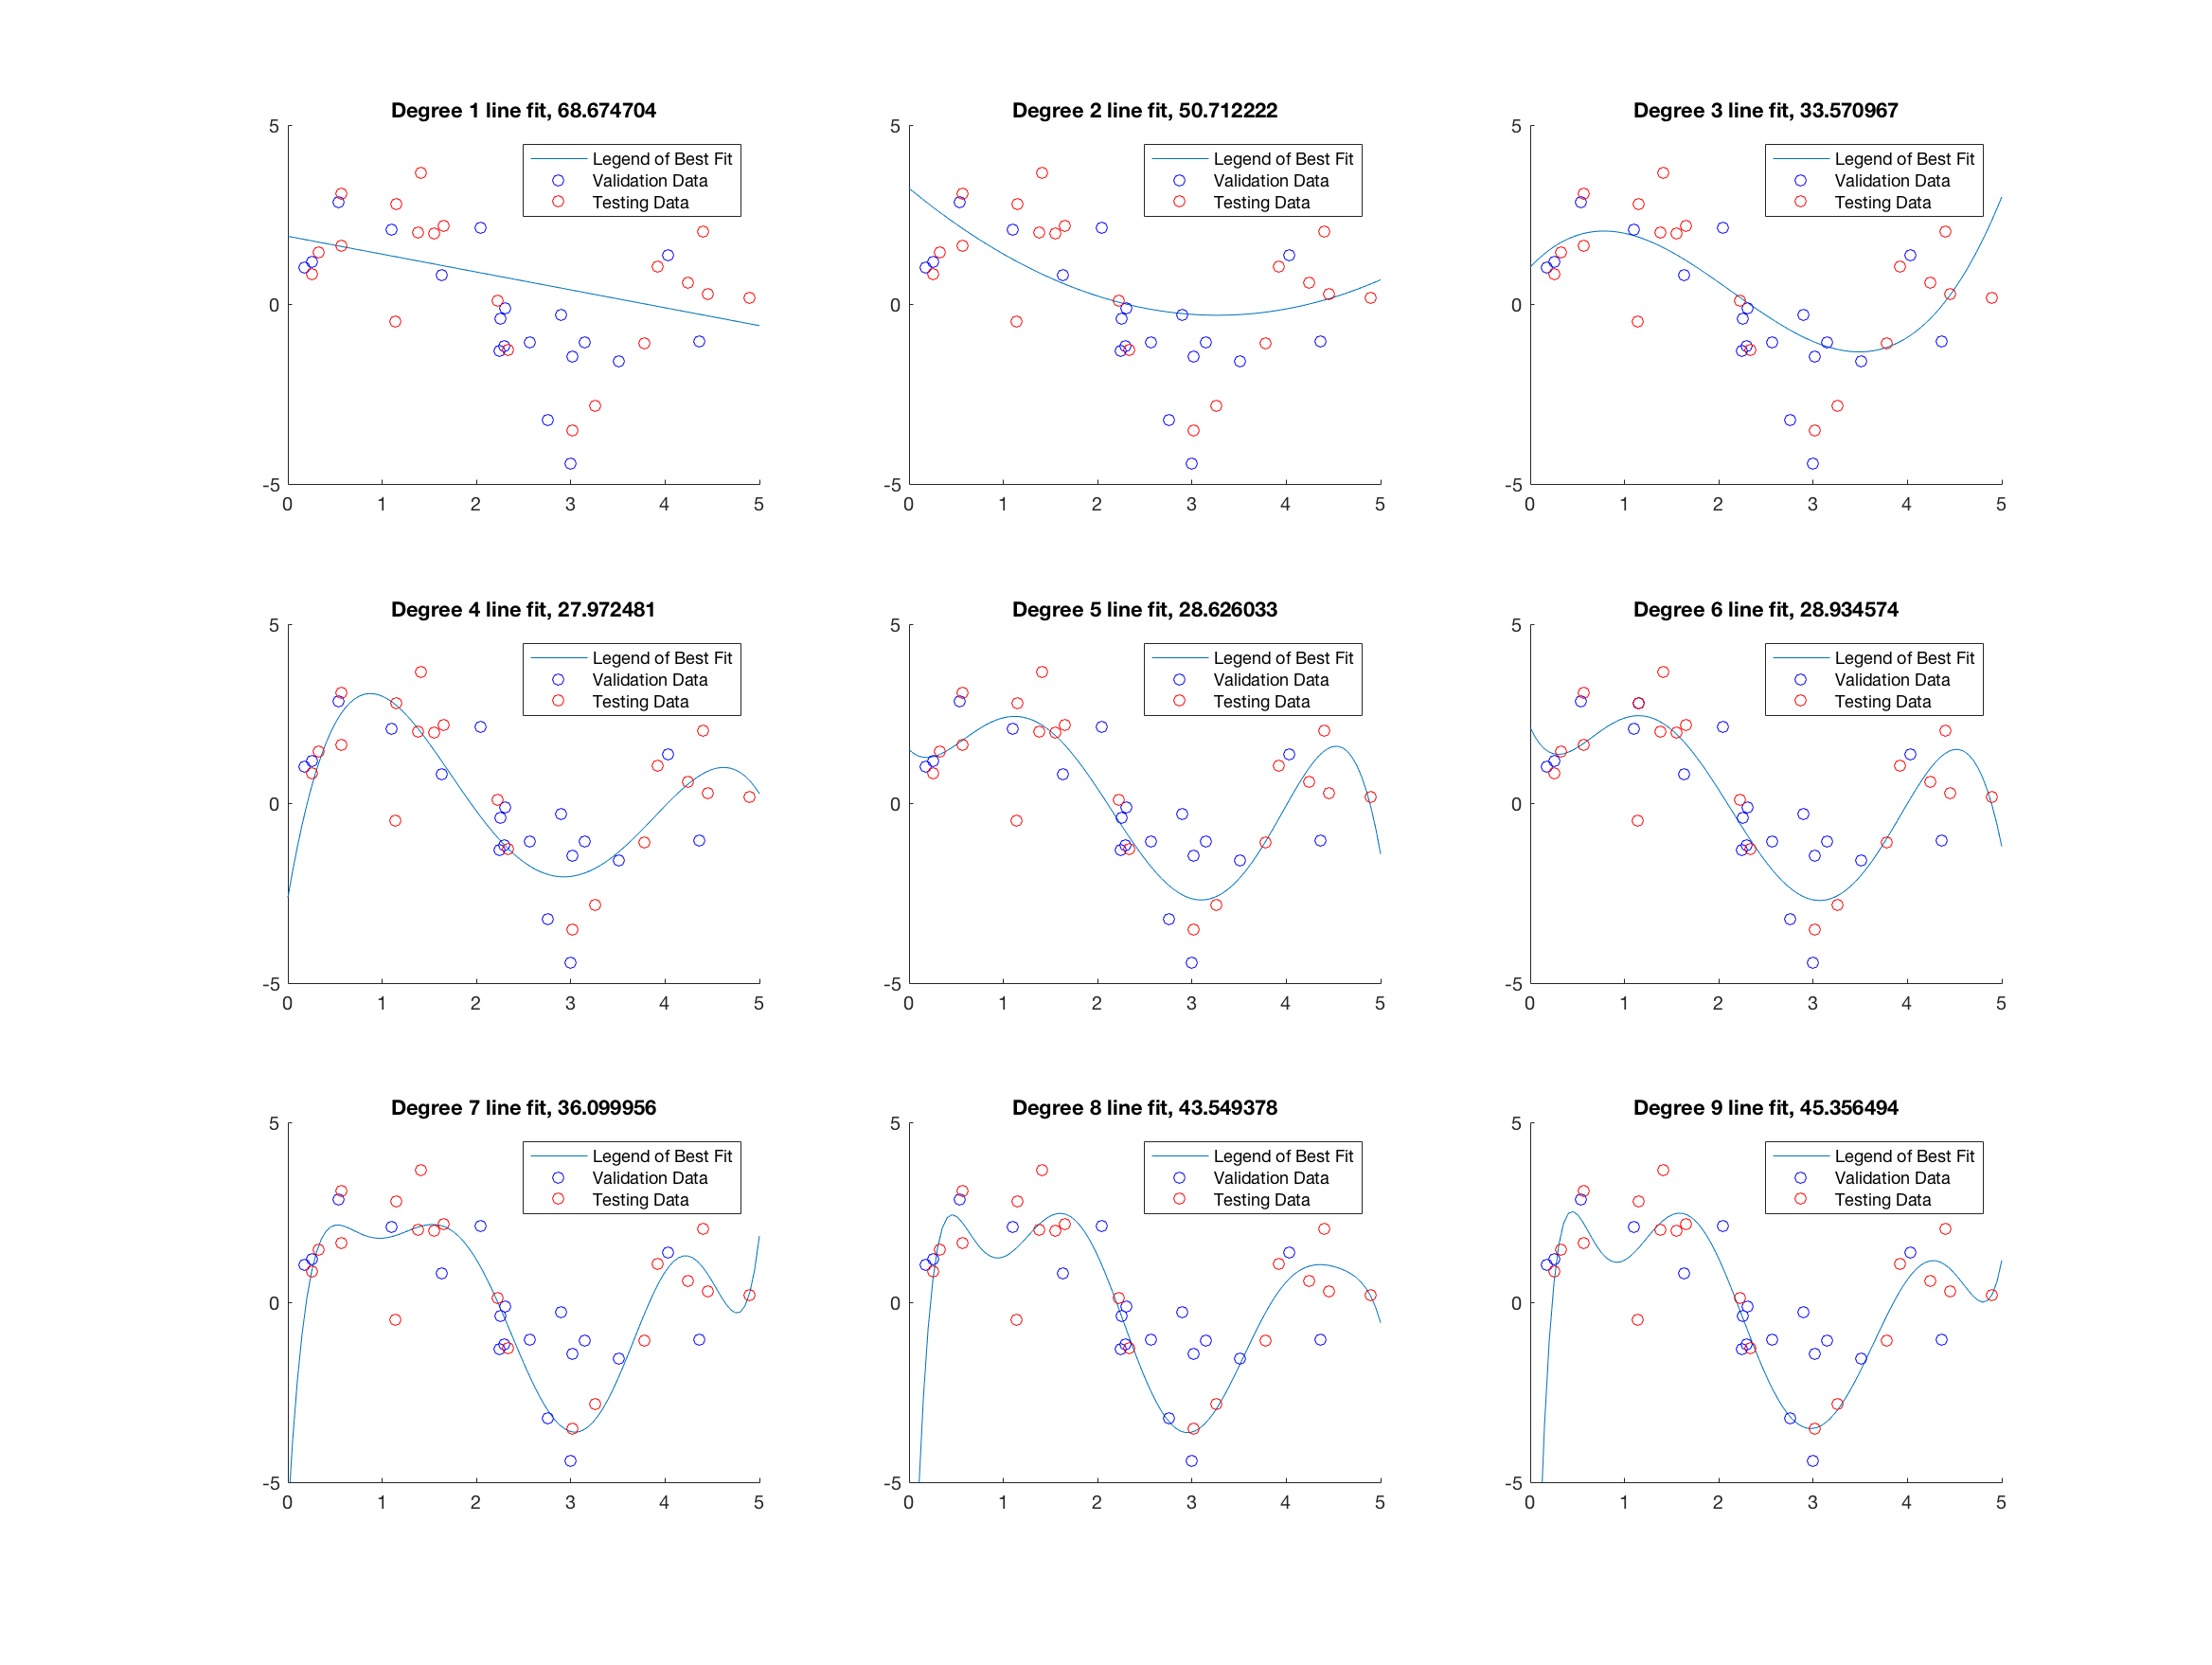
\includegraphics[width=\linewidth]{../../pracs/week3/images/q1_lines_of_best_fit}
    \centering
    \caption{Lines of best fit}
\end{figure}

\begin{figure}[H]
    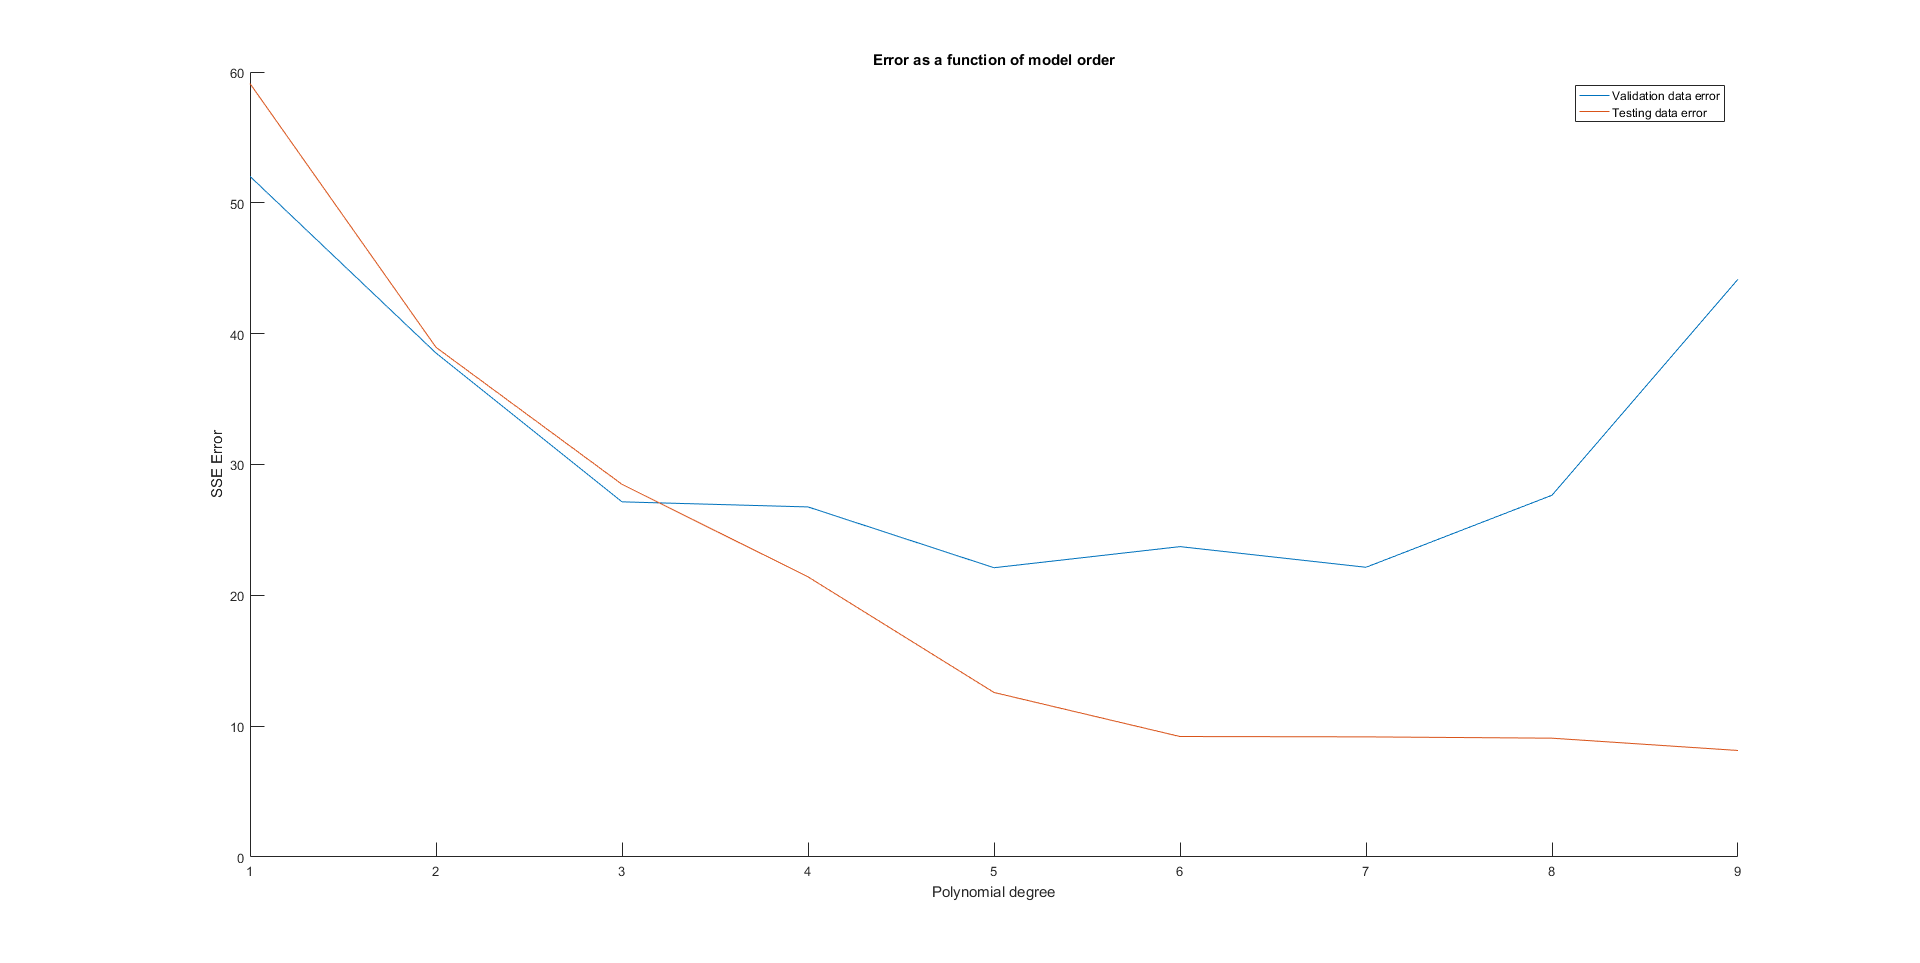
\includegraphics[width=\linewidth]{../../pracs/week3/images/q1_err_vs_degree}
    \centering
    \caption{Error vs Polynomial Degree}
\end{figure}

\section*{Question 2.4}

\lstinputlisting[language=Matlab]{../../pracs/week3/q4.m}

\begin{figure}[H]
    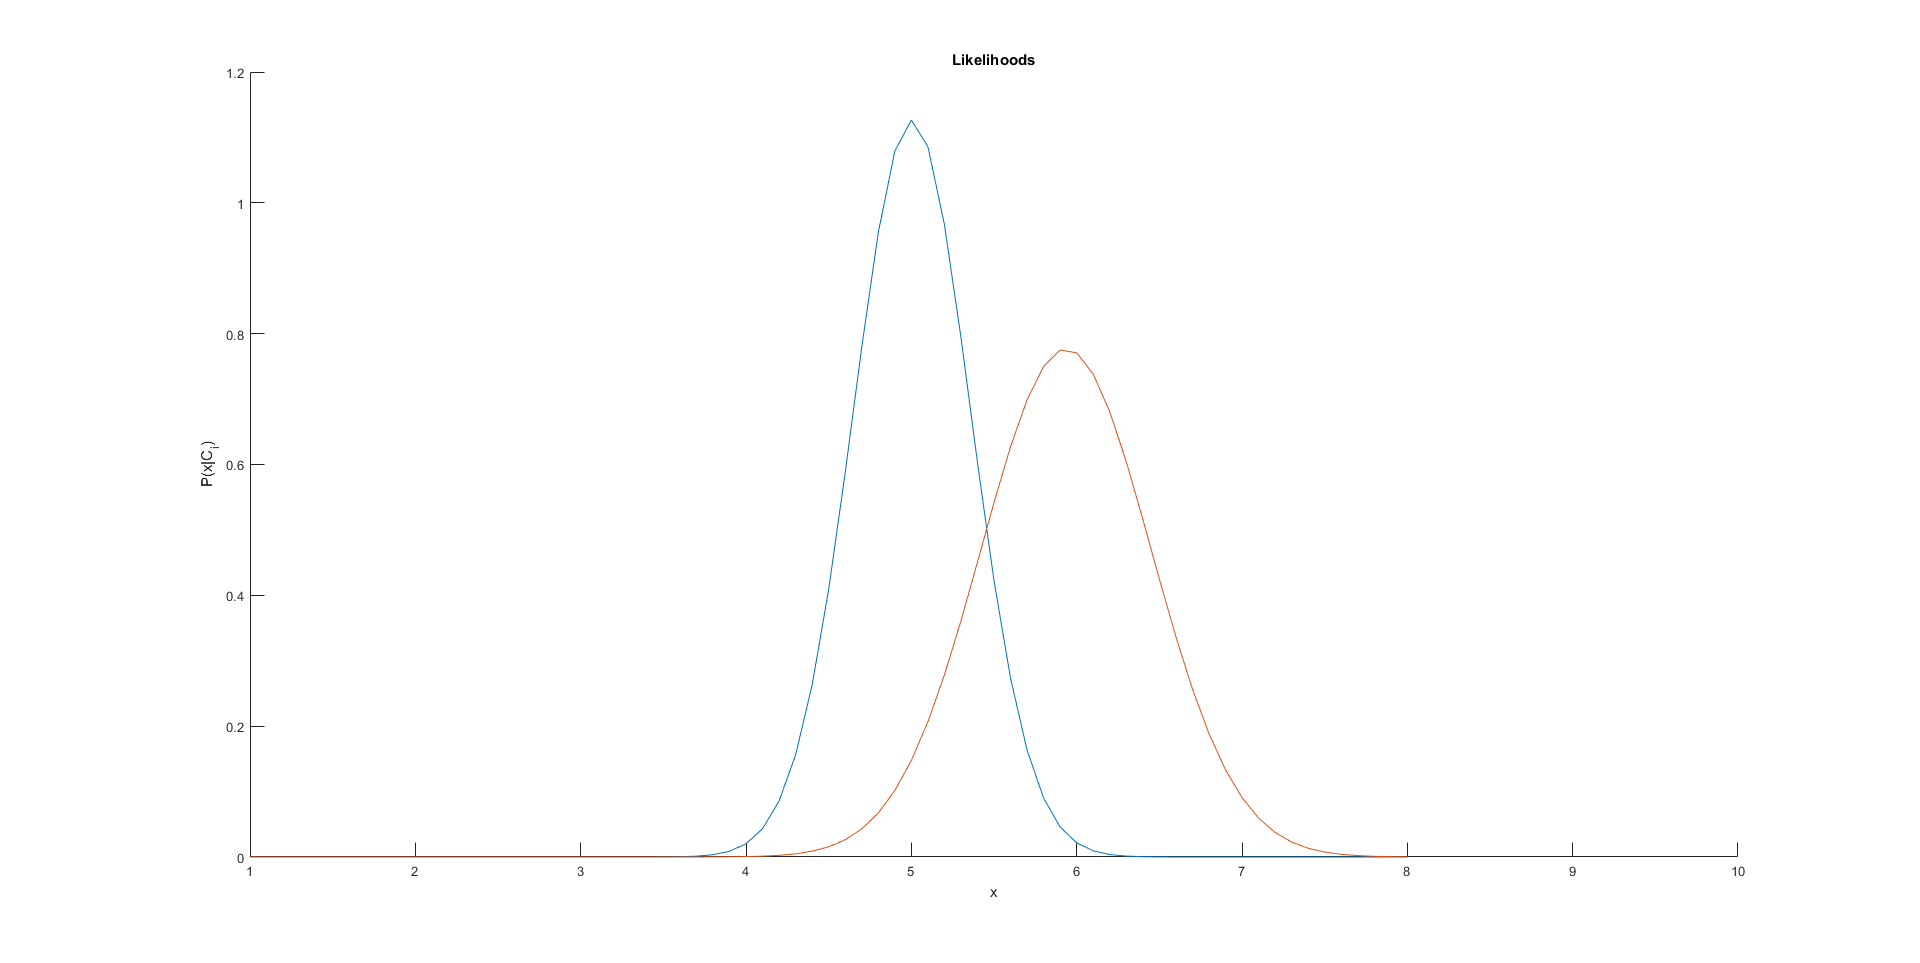
\includegraphics[width=\linewidth]{../../pracs/week3/images/q4_likelihoods}
    \centering
    \caption{Likelihoods}
\end{figure}

\begin{figure}[H]
    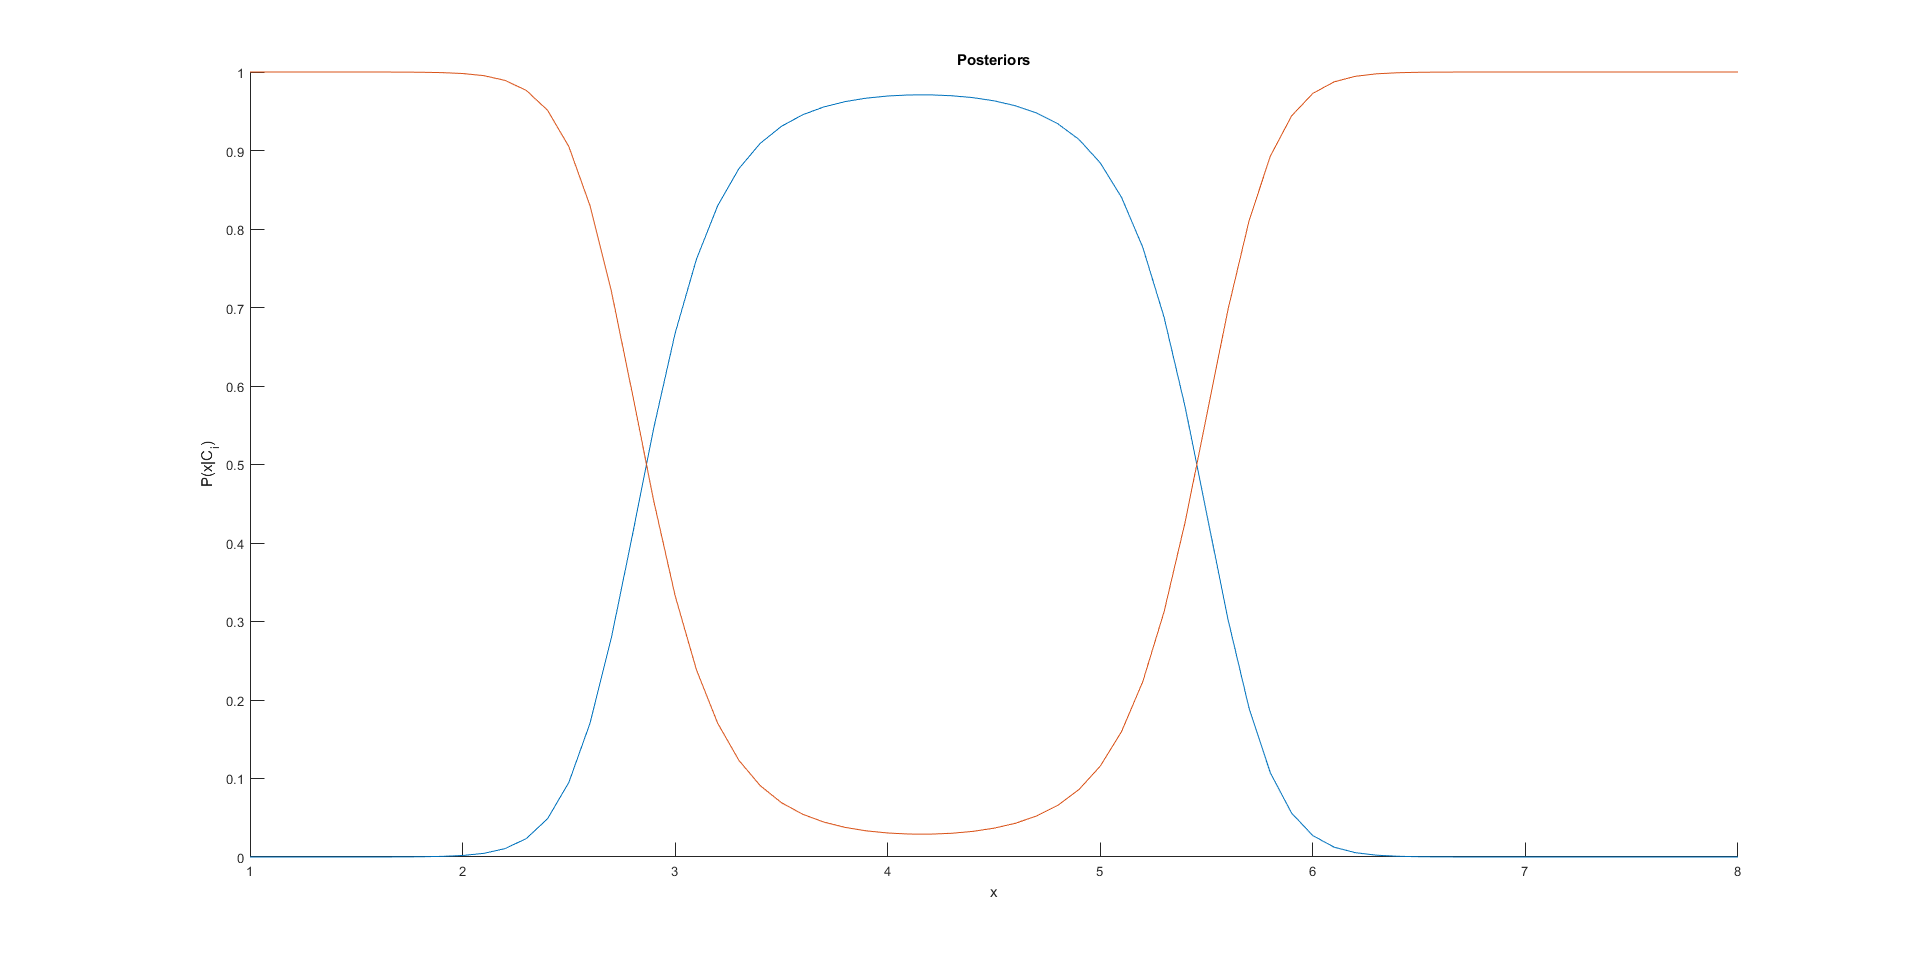
\includegraphics[width=\linewidth]{../../pracs/week3/images/q4_posteriors}
    \centering
    \caption{Posteriors}
\end{figure}

\section*{Question 3.1}

\section*{Question 3.2}

\section*{Question 3.5}

\end{document}
